\section{Поверхности второго порядка}

Пусть задана плоскость, а в ней линия, заданная функцией f(x, z). Начнем вращать линия вокруг оси Oz. Каждая точка на линии описывает окружность радиусом |x|, при этом z сохраняется, но изменяется координата по y, т.е. |x| = $\sqrt{x^2 + y^2}$ $\Longrightarrow$
\[
f(\sqrt{x^2 + y^2}, z)\cdot f(-\sqrt{x^2 + y^2}, z) = 0 - \underline{\text{уравнение поверхности вращения}}
\]

Рассмотрим линию в пространстве и вектор $\overline{a}\neq\overline{0}$. Назовем линию \textit{направляющей} и проведем через каждую точку, лежащую на ней, \textit{образующие}, параллельные $\overline{a}$. Таким образом, получим \underline{цилиндрическую поверхность}.\\

\underline{Коническая поверхность} образована прямыми, проходящими через все точки направляющей кривой и точку, лежащую вне этой кривой.\\

\begin{definition}
    \textit{Поверхность второго порядка} задается следующим образом
    \[
    \begin{cases}
        A_1x^2 + A_2y^2 + A_3z^2 + 2A_4xy + 2A_5xz + 2A_6yz + 2A_7x + 2A_8y + 2A_9z + A_{10} = 0\\
        A_1^2 + A_2^2 + A_3^2 + A_4^2 + A_5^2 + A_6^2 > 0
    \end{cases}
    \]
\end{definition}

Всего 17 типов поверхностей второго порядка.\\

Прямая и поверхность второго порядка имеют либо 0, либо 1, либо 2 общие точки, либо прямая целиком принадлежит поверхности.\\

\begin{definition}
    Прямая, целиком лежащая на поверхности, называется \textit{прямолинейной образующей} этой поверхности.
\end{definition}

\subsection{Эллипсоид}

\begin{wrapfigure}{l}{0.5\textwidth}
    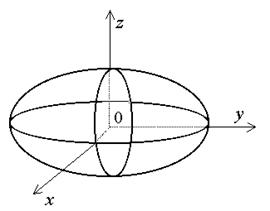
\includegraphics[width=1.0\linewidth]{images/эллипсоид.jpg}
\end{wrapfigure}

\tab\\

\underline{Уравнение:}
\[
\dfrac{x^2}{a^2} + \dfrac{y^2}{b^2} + \dfrac{z^2}{c^2} = 1 \tab a, b, c > 0
\]

\underline{Основные сечения:}
\begin{itemize}
    \item Эллипсы
\end{itemize}

\underline{Свойства:}
\begin{itemize}
    \item Центральная и осевая симметрии
    \item Ограниченность
    \item Если 2 коэффициента равны, то это эллипсоид вращения
    \item Если все коэффициенты совпадают, то это сфера
    \item Нет прямолинейных образующих
\end{itemize}

\subsection{Эллиптический параболоид}
\begin{wrapfigure}{l}{0.5\textwidth}
    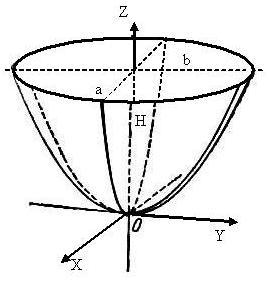
\includegraphics[width=1.0\linewidth]{images/эллиптический параболоид.JPG}
\end{wrapfigure}

\tab\\

\underline{Уравнение:}
\[
\dfrac{x^2}{a^2} + \dfrac{y^2}{b^2} = 2z \tab a, b > 0
\]

\underline{Основные сечения:}
\begin{itemize}
    \item Эллипс - 1 сечение
    \item Параболы - 2 сечения
\end{itemize}

\underline{Свойства:}
\begin{itemize}
    \item Неограниченность
    \item Осевая симметрия
    \item Если a = b, то это параболоид вращения
    \item Нет прямолинейных образующих
\end{itemize}
\tab\\ \tab\\ \tab\\ \tab\\
\subsection{Гиперболический параболоид}

\begin{wrapfigure}{l}{0.5\textwidth}
    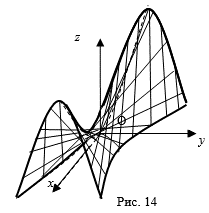
\includegraphics[width=0.7\linewidth]{images/гиперболический параболоид.png}
\end{wrapfigure}

\tab\\

\underline{Уравнение:}
\[
\dfrac{x^2}{a^2} - \dfrac{y^2}{b^2} = 2z \tab a, b > 0
\]

\underline{Основные сечения:}
\begin{itemize}
    \item Параболы - 2 сечения
    \item Гипербола - 1 сечение
\end{itemize}

\clearpage
\underline{Свойства:}
\begin{itemize}
    \item  Неограниченность
    \item Осевая симметрия
    \item Через каждую точку можно провести 2 прямолинейные образующие
\end{itemize}


\subsection{Однополостный гиперболоид}

\begin{wrapfigure}{l}{0.5\textwidth}
    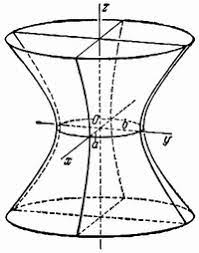
\includegraphics[width=0.7\linewidth]{images/однополостный гиперболоид.jpeg}
\end{wrapfigure}

\underline{Уравнение:}
\[
\dfrac{x^2}{a^2} + \dfrac{y^2}{b^2} - \dfrac{z^2}{c^2} = 1 \tab a, b, c > 0
\]

\underline{Основные сечения:}
\begin{itemize}
    \item Эллипс - 1 сечение
    \item Гиперболы - 2 сечения
\end{itemize}

\underline{Свойства:}
\begin{itemize}
    \item Неограниченность
    \item Центральная и осевая симметрии
    \item Если 2 коэффициента равны, то это гиперболоид вращения
    \item Через каждую точку можно провести 2 прямолинейные образующие
\end{itemize}

\tab\\ \tab\\
\subsection{Конус}

\begin{wrapfigure}{l}{0.5\textwidth}
    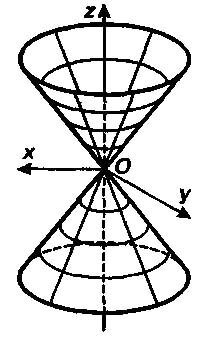
\includegraphics[width=0.5\linewidth]{images/конус.jpg}
\end{wrapfigure}

\tab\\

\underline{Уравнение:}
\[
\dfrac{x^2}{a^2} + \dfrac{y^2}{b^2} - \dfrac{z^2}{c^2} = 0 \tab a, b, c > 0
\]

\underline{Основные сечения:}
\begin{itemize}
    \item Эллипс
    \item Парабола
    \item Гипербола
\end{itemize}
\clearpage
\underline{Свойства:}
\begin{itemize}
    \item Неограниченность
    \item Центральная и осевая симметрии
    \item Если 2 коэффициента равны, то это гиперболоид вращения
    \item Через каждую точку можно провести 1 прямолинейную образующую, через вершину проходят все линейные образующие
\end{itemize}

\subsection{Двуполостный гиперболоид}

\begin{wrapfigure}{l}{0.5\textwidth}
    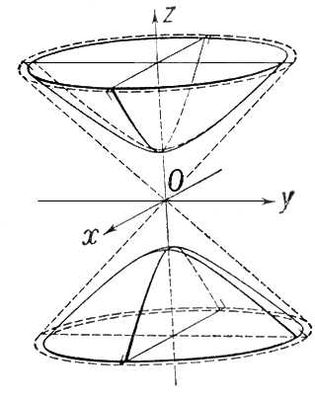
\includegraphics[width=.7\linewidth]{images/двуполостный гиперболоид.jpg}
\end{wrapfigure}

\tab\\ 

\underline{Уравнение:}
\[
-\dfrac{x^2}{a^2} - \dfrac{y^2}{b^2} + \dfrac{z^2}{c^2} = 1 \tab a, b, c > 0
\]

\underline{Основные сечения:}
\begin{itemize}
    \item Эллипс - 1 сечение
    \item Гипербола - 2 сечения
\end{itemize}

\underline{Свойства:}
\begin{itemize}
    \item Неограниченность
    \item Центральная и осевая симметрии
    \item Нет прямолинейных образующих
\end{itemize}

\tab\\ \tab\\ \tab\\
\subsection{Параболический цилиндр}

\begin{wrapfigure}{l}{0.5\textwidth}
    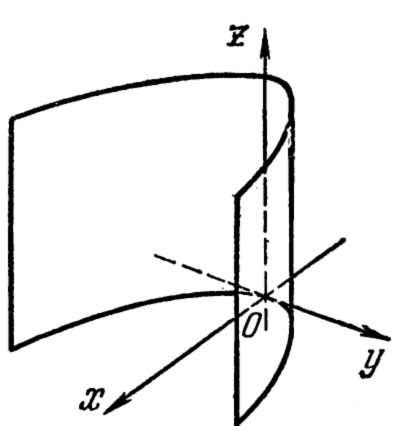
\includegraphics[width=.5\linewidth]{images/параболический цилиндр.png}
\end{wrapfigure}

\tab\\

\underline{Уравнение:}
\[
y^2 = 2px
\]
\clearpage
\subsection{Гиперболический цилиндр}

\begin{wrapfigure}{l}{0.5\textwidth}
    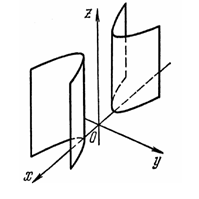
\includegraphics[width=.5\linewidth]{images/гиперболический цилиндр.png}
\end{wrapfigure}

\tab\\

\underline{Уравнение:}
\[
\dfrac{x^2}{a^2} - \dfrac{y^2}{b^2} = 1
\]

\tab\\ \tab\\ \tab\\ \tab\\ 
\subsection{Эллиптический цилиндр}

\begin{wrapfigure}{l}{0.5\textwidth}
    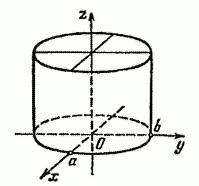
\includegraphics[width=.5\linewidth]{images/эллиптический цилиндр.jpeg}
\end{wrapfigure}

\tab\\

\underline{Уравнение:}
\[
\dfrac{x^2}{a^2} + \dfrac{y^2}{b^2} = 1
\]


